\section{Face Recognition}
The first computer based face recognition was made in 1973. This was based on a feature approach, meaning the program identifies basic face features such as mouth, eye, and nose placement. 
From here three different types of approaches emerged, namely a holistic, feature extraction and a hybrid approach. 

The holistic approach encodes the entirety of a face and then identifies using template-matching, the feature extraction approach extracts a defined amount of features from the face, whereas the hybrid method uses both template-matching and feature extraction \citep{Wechsler2007}.
In 1990, \gls{pca} was introduced for holistic face recognition. The \gls{pca} approach makes use of eigenfaces, each eigenface represents a principal component in which a face is encoded. But as \cite{Wechsler2007} claims, \gls{lda} is a more effective suitable approach for face identification and authentication. Another holistic approach is using \gls{svm} for face recognition \citep{Wechsler2007}.

The feature approach gave way for what is now known as recognition-by-parts, which uses the features and a global structure to link these features. A structure for linking 2D features is the \gls{hmm}. \gls{pca} is also used in this approach, but is used to model shape or texture of the face.

In the late 2000s deep learning was introduced with representation-learning methods with multiple levels of representation. By feeding raw data and finding and emphasising on the important aspects of the data and suppressing the unimportant ones, higher level classification is possible \citep{LeCun2015}. This is done with several \textit{hidden layers}. The more layers there are, the deeper a network is said to be. 

In the following some of the state of the art deep learning networks for face recognition are presented.

\subsection{DeepID}
\gls{deepid} is a \gls{cnn} which aims to use feature extraction for face identification and verification. It detects five facial landmarks; the two eye centres, the nose tip, and the two mouth corners. The network is made of four convolutional layers with max-pooling, which are used to extract features hierarchically. These are followed by the fully-connected \gls{deepid} layer and a softmax output layer to indicate identity classes. The feature extraction and face recognition is done in two steps, where the first step, feature extraction, is learned with the target of face identification \citep{deepID2014}.

In the \gls{cnn}s the neuron number of the last hidden layer in the network is much smaller than that of the output layer. This is done, to better classify faces \citep{deepID2014}. The network extracts low-level features in the bottom layers, where feature numbers decreases for each layer. In opposition, the high-level features are formed in the top layers. An overview of the network structure is shown in \autoref{fig:deepid_convnet}.

The network is tested using the \gls{lfw} database. This database is images of faces from different angles and scenarios consisting of 13.233 images from 5749 subjects. However, only 1680 of the subjects are sampled more than twice \citep{lfw2007}. It achieves $97.45\%$ accuracy on this dataset, requiring weakly aligned faces \citep{deepID2014}.

\begin{figure}[h]
	\centering
	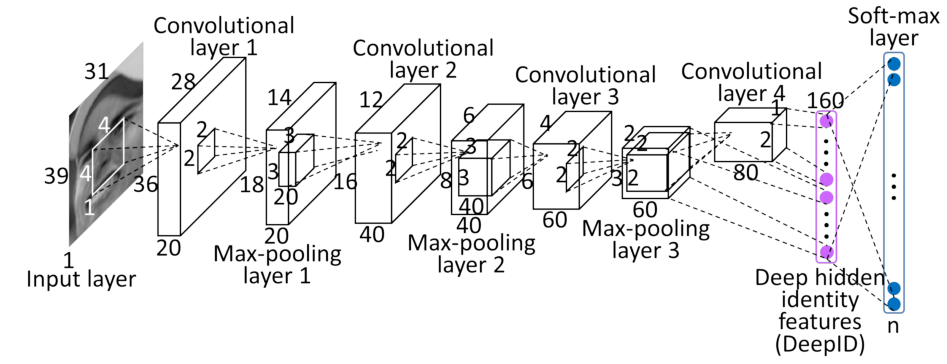
\includegraphics[width=\textwidth]{figures/deepid_convnet}
	\caption{Structure of the \gls{cnn} used in \gls{deepid} \citep{deepID2014}}
	\label{fig:deepid_convnet}
\end{figure}

\subsection{DeepID2}
\gls{deepid2} is an expansion upon \gls{deepid} and is a deep \glsentrylong{cnn} used for face identification and verification. This is done by using feature extraction.

Just like \gls{deepid}, \gls{deepid2} uses four convolutional layers but only the first three uses max-pooling. It uses 400 face patches instead of 60 \citep{deepID2014,sun2014} and detects 21 landmarks of the face.

The \gls{deepid2} layer is after the four convolutional layers. This layer is learned under two supervisory signals. The first is identification classifying the images into identities. The second is face verification which manipulates the \gls{deepid2} data to be similar to a matching identity should this be the same. \autoref{fig:deepid2_convnet} shows the structure af the \gls{deepid2} network.

\gls{deepid2} also uses the \gls{lfw} database and achieves a $99.15\%$ accuracy.

\begin{figure}[h]
	\centering
	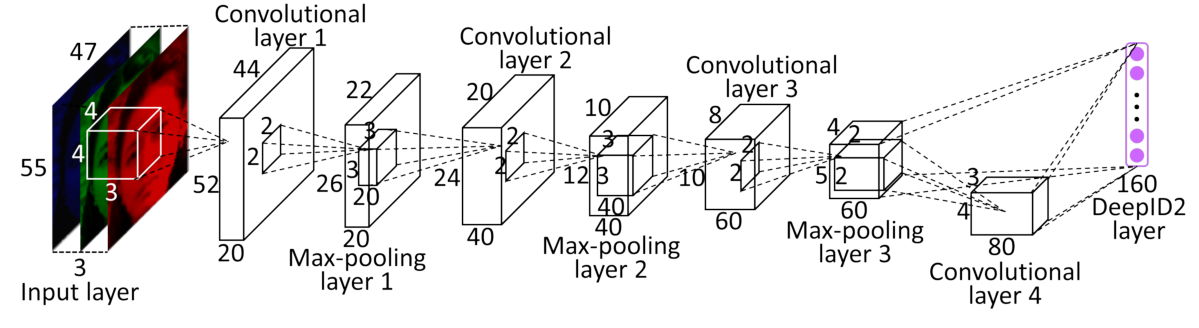
\includegraphics[width=\textwidth]{figures/deepid2_convnet}
	\caption{Structure of the \gls{cnn} used in \gls{deepid2} \citep{sun2014}}
	\label{fig:deepid2_convnet}
\end{figure}

\subsection{DeepID3}
DeepID3 is a further expansion of both \gls{deepid} and \gls{deepid2} but is also drawing on some from elements from VGG net and GoogleNet \citep{sun2015}. The qualities from these two networks is the use of stacked convolution and inception layers. DeepID3 is in general a deeper network than \gls{deepid2} and its expansion \gls{deepid2}+. However, DeepID3 resembles \gls{deepid2} in the use of adding supervisory signals to early layers.

\cite{sun2015} proposes two different networks with DeepID3. One is using eight convolutional layers with max pooling after every other convolutional layer. The second network has four convolutional layers with max pooling after every other, following are five inception layers. These two networks are shown in \autoref{fig:deepid3_net}.

DeepID3 is also tested on the \gls{lfw} dataset with an accuracy of $99.52\%$ which is an increase in accuracy compared to \gls{deepid2}, but as stated in \cite{sun2015} it is not an improvement of \gls{deepid2}+.

\begin{figure}[h]
	\centering
	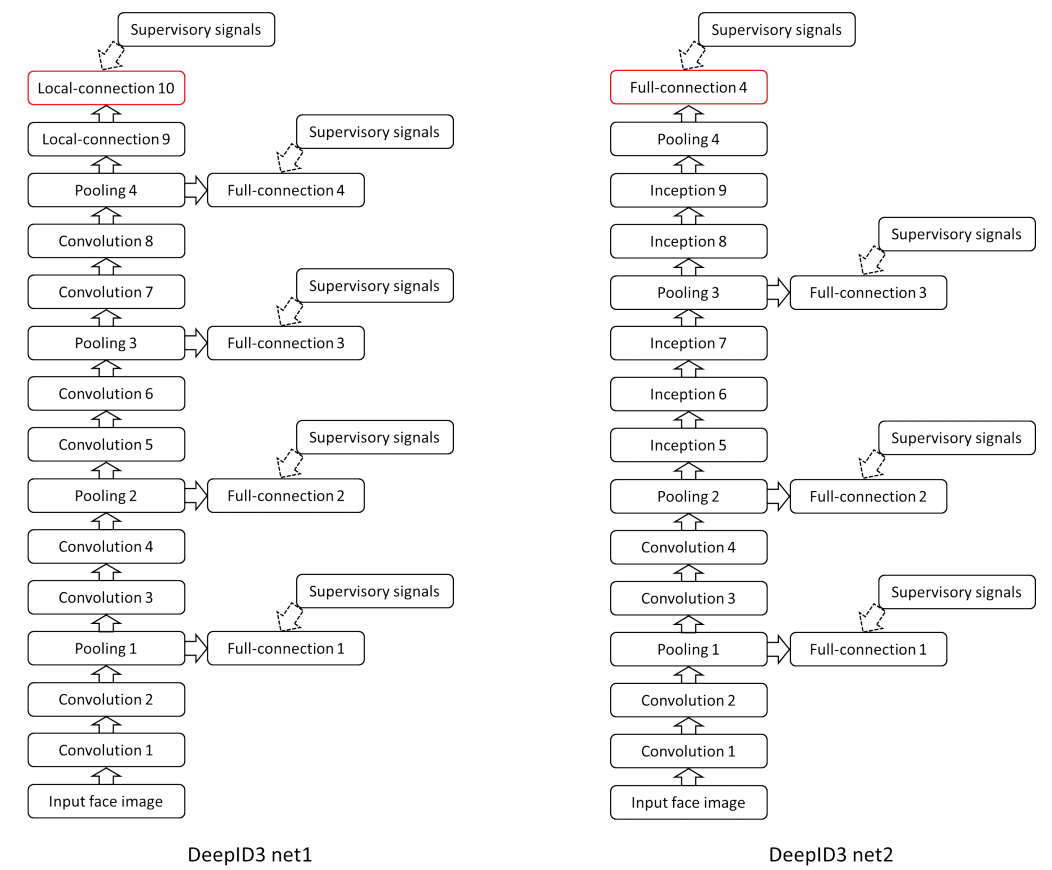
\includegraphics[width=\textwidth]{figures/deepid3_net}
	\caption{Structure of the \gls{cnn}s used in DeepID3 \citep{sun2015}}
	\label{fig:deepid3_net}
\end{figure}